% This LaTeX was auto-generated from MATLAB code.
% To make changes, update the MATLAB code and export to LaTeX again.

\documentclass{article}

\usepackage[utf8]{inputenc}
\usepackage[T1]{fontenc}
\usepackage{lmodern}
\usepackage{graphicx}
\usepackage{color}
\usepackage{hyperref}
\usepackage{amsmath}
\usepackage{amsfonts}
\usepackage{epstopdf}
\usepackage[table]{xcolor}
\usepackage{matlab}
\usepackage[paperheight=795pt,paperwidth=614pt,top=72pt,bottom=72pt,right=72pt,left=72pt,heightrounded]{geometry}

\sloppy
\epstopdfsetup{outdir=./}
\graphicspath{ {./Difuzija_vezba_media/} }

\begin{document}

\matlabtitle{Osnovi biofizike: Vežba difuzija}

\matlabheading{Uvod }

\begin{par}
\begin{flushleft}
Čuveni teorijski fizičar Albert Ajnštajn (tvorac specijalne teorije relativnosti) je 1905. godine modelovao difuziju čestica polena u vodi. Ovo je bio jedan od njegovih prvih velikih naučnih doprinosa (iste godine je objavio i rad o specijalnoj teoriji relativnosti). Francuski naučnik Jean-Baptiste Perrin je 1908. godine eksperimentalno potvrdio Ajnštajnovu teoriju, za šta je 1926. godine dobio i Nobelovu nagradu. Iako nam se postojanje atoma i molekula danas čini očiglednim, to nije bio slučaj početkom 20. veka, a poklapanje eksperimenta i teorije o difuziji je poslužilo kao ubedljiv dokaz o njihovom postojanju. Razvoj molekulske i atomske teorije je utro put i kasnijem razvoju molekularne biologije. Ova vežba je direktno zasnovana na podacima Jean Perrin i cilj nam je da kroz nju direktno potvrdimo zakon difuzije, kao i da primenom statističke analize odredimo konstantu difuzije.   
\end{flushleft}
\end{par}

\matlabheading{Deo 1: Analiza eksperimentalnih podataka Braunovog kretanja iz Jean Perrin rada}

\matlabheadingtwo{1) Učitavanje i upoznavanje sa podacima}

\begin{par}
\begin{flushleft}
Podaci iz Joan Perrin eksperimenta se nalaze u .mat fajlu "g26perrindata". Prvo ucitavamo Jean Perrin Brownian motion diffusion data:
\end{flushleft}
\end{par}

\begin{matlabcode}
clear all ;
load g26perrindata.mat
whos % prikazuje varijable koje su ucitane
\end{matlabcode}
\begin{matlaboutput}
  Name              Size            Bytes  Class     Attributes

  README            1x93              186  char                
  perrindata      508x2              8128  double              
\end{matlaboutput}
\begin{matlabcode}
README %kratak opis podataka
\end{matlabcode}
\begin{matlaboutput}
README = 'Perrin's data on Brownian motion. x,y values of endpoints of 508 random walks, in micrometers'
\end{matlaboutput}
\begin{matlabcode}
perrindata(1:5,:) %prikaz dela podataka, odnosno prvih 5 vrsta
\end{matlabcode}
\begin{matlaboutput}
ans = 5x2    
   13.8237    9.4710
    9.9175   10.8331
  -10.0919   14.5292
  -10.9304   12.8787
   -8.3908   14.0763

\end{matlaboutput}

\begin{par}
\begin{flushleft}
Iz gornjeg prikaza vidimo da su podaci slozeni u dve kolone, prva odgovara $\delta x$ (relativni pomeraj čestice u x pravcu) druga odgovara $\delta y$ (relativni pomeraj y pravcu). Pod relativnim pomerajem se podrazumeva promena položaja čestice u odnosu na prethodno izmerenu poziciju, pri čemu su u tom eksperimentu meranja vršena svakih 30s. Ukupan broj raspoloživih meranja možemo videti ako prikažemo dimenziju matrice sa podacima:
\end{flushleft}
\end{par}

\begin{matlabcode}
size(perrindata)
\end{matlabcode}
\begin{matlaboutput}
ans = 1x2    
   508     2

\end{matlaboutput}

\matlabheadingtwo{2) Analiza distribucije pomeraja:}

\begin{par}
\begin{flushleft}
Od relativnih pomeraja u x i y pravcu koji su dati u matrici, prvo želimo da vizuelno prikažemo putanju, odnosno kumulativne pomeraje čestice: 
\end{flushleft}
\end{par}

\begin{matlabcode}
xt = cumsum(perrindata(:,1)) ; %kumulativni pomeraj cestice duz x

yt = cumsum(perrindata(:,2)) ; %kumulativni pomeraj cestice duz y

figure()

plot( xt , yt , '-or' )
xlabel("Položaj duž x ose (nm)") ;
ylabel("Položaj duž y ose (nm)") ;
title('Izmerena trajektorija čestice u Perinovom eksperimentu') ;
\end{matlabcode}
\begin{center}
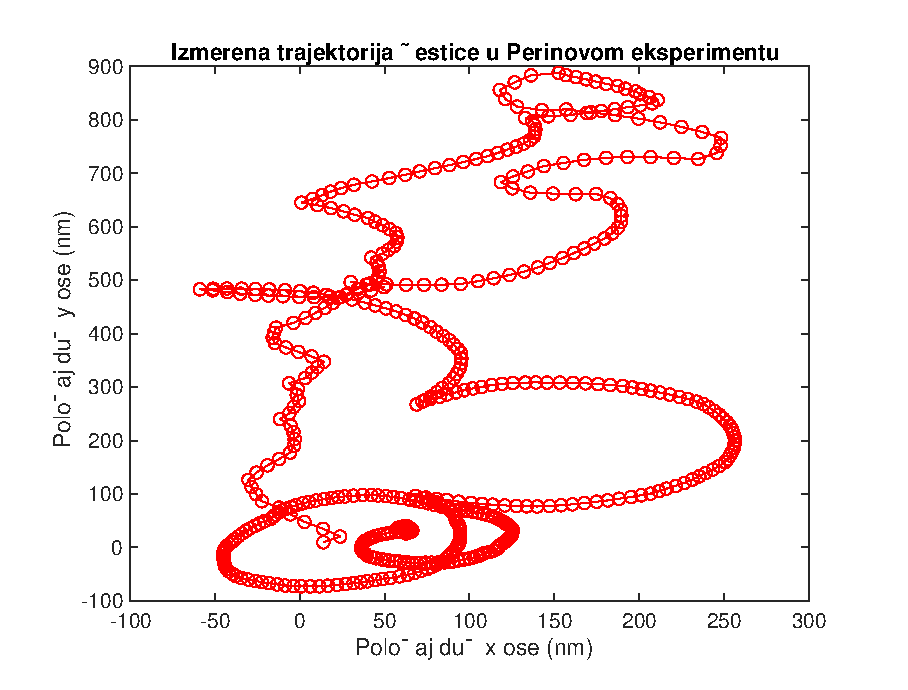
\includegraphics[width=\maxwidth{56.196688409433015em}]{figure_0.eps}
\end{center}

\begin{par}
\begin{flushleft}
Iz prikazane trajektorije vidimo da su sukcesivni pomeraji različiti (neki manji a neki veći), pa nam je sledeći cilj da nadjemo raspodelu ovih pomeraja. Posmatraćemo zasebno dve raspodele, jednu duž x a drugu duž y ose ( videćemo da su praktično identične). Ajnštajnova teorija difuzije predvidja da ove distribucije odgovaraju Gausovoj raspodeli, pa da bi to potvrdili direktno iz podataka na empirijske distribucije fitujemo Gausove krive.
\end{flushleft}
\end{par}

\begin{matlabcode}
%deltaLsquare = sqrt( perrindata(:,1).^2 + perrindata(:,2).^2 ) ;
deltaX = perrindata(:,1)   ;
deltaY = perrindata(:,2)   ;
\end{matlabcode}

\begin{par}
\begin{flushleft}
Crtamo histogram (raspodelu) relativnih pomeraja zasebno za $\delta x$ i $\delta y$:
\end{flushleft}
\end{par}

\begin{matlabcode}
figure()  ;

tiledlayout('vertical')  ;

nexttile  ;

histogram( deltaX , 'Normalization', 'pdf')  ; %Empirijska distribucija x pomeraja


[x_values , y_values , SigmaX ] = fitGauss( deltaX )  ;  % pored x i y vrednosti fitovane krive, funkcija daje i standardnu devijaciju (sigmaX) fitovane distribucije

hold on  ;

plot(x_values, y_values, 'r', 'LineWidth', 2) ; % Crtanje fitovane Gausove distribucije

xlabel("Relativni pomeraji duž x ose") ;
ylabel('Raspodela pomeraja') ;
title('Raspodela pomeraja i fit normalne distribucije za \deltax') ;
legend('Empirijska distribucija', 'Gausov fit') ;
hold off

nexttile ;

histogram( deltaY , 'Normalization', 'pdf')  ;  %Empirijska distribucija y pomeraja

hold on ;

[x_values , y_values , sigmaY ] = fitGauss( deltaY )  ; % pored x i y vrednosti fitovane krive, funkcija daje i standardnu devijaciju (sigmaY) fitovane distribucije

plot(x_values, y_values, 'r', 'LineWidth', 2);

hold off ;

xlabel("Relativni pomeraji duž y ose") ;
ylabel('Raspodela pomeraja') ;
title('Raspodela pomeraja i fit normalne distribucije za \deltay') ;
legend('Empirijska distribucija', 'Gausov fit') ;
\end{matlabcode}
\begin{center}
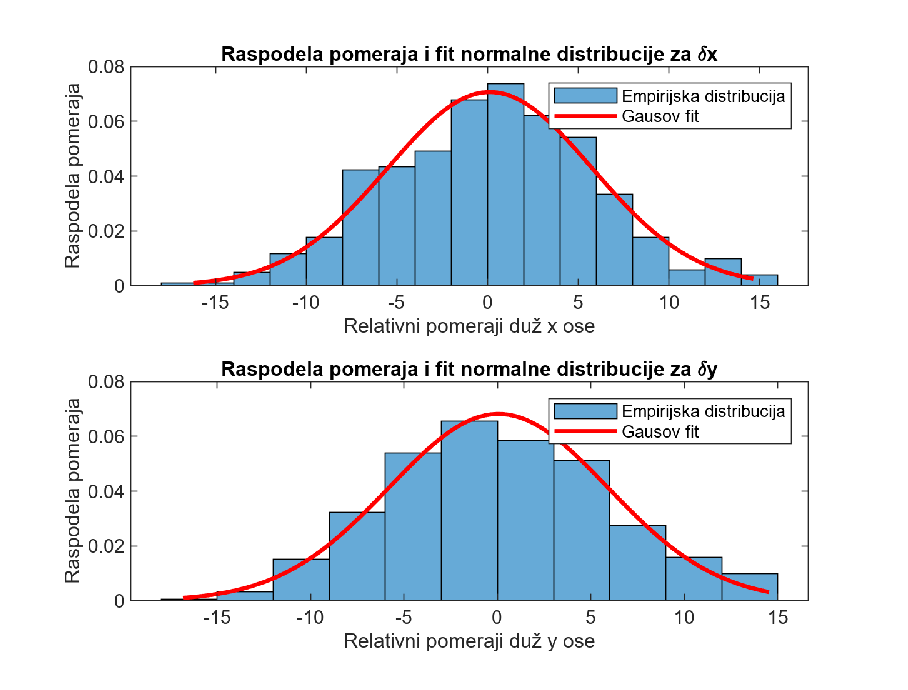
\includegraphics[width=\maxwidth{56.196688409433015em}]{figure_1.eps}
\end{center}

\begin{par}
\begin{flushleft}
Vidimo da u oba slučaja ("x" ili "y" osa) dobijamo raspodelu koja ima oblik "zvona", dakle koja je centrirana na nuli, ali i sa značajnom varijabilnošću (disperzijom). Ova varijabilnost potiče od toga što se u svakom intervalu od 30s izmedju sukcesivnih merenja dešava veoma velik broj sudara izmedju posmatrane čestice i molekula vode. Pri svakom sudaru čestica ima podjednaku verovatnoću da se pomeri nalevo ili nadesno, usled čega su obe raspodele centrirane na nuli, dok je širina (standardna devijacija) distribucije povezana sa verovatnoćom da česticu nadjemo na odredjenom rastojanju od nule. Kao što je i očekivano, raspodela empirijskih podataka se dobro slaže sa Gausovom raspodelom.  
\end{flushleft}
\end{par}

\matlabheadingtwo{3) Odredjivanje konstante difuzije:  }

\begin{par}
\begin{flushleft}
Na osnovu fitova Gausove distribucije dobijenih u prethodnom delu vežbe cilj nam je da odredimo konstantu difuzije (D) iz Perrinovih izmerenih podataka. Za to poredimo zakon 1D difuzije: 
\end{flushleft}
\end{par}

\begin{par}
$$P(x,t)=\frac{1}{\sqrt{4\pi Dt}}\exp \left(-\frac{x^2 }{4Dt}\right)$$
\end{par}

\begin{par}
\begin{flushleft}
sa oblikom fitovane Gausove distribucije:
\end{flushleft}
\end{par}

\begin{par}
$$P(x,t)=\frac{1}{\sqrt{2\pi }\sigma }\exp \left(-\frac{x^2 }{2\sigma^2 }\right)$$
\end{par}

\begin{par}
\begin{flushleft}
Poredjenjem dobijamo dobro poznatu relaciju $\sigma^2 =2Dt$ koja se česti piše i u obliku: $\delta x^2 =2Dt$. Odatle dobijamo $D=\sigma^2 /(2t)$, pa znajući t=30s i na osnovu standardne devijacije dobijene u prethodnom zadatku (biramo da odredimo D iz x ose, ali se veoma slična vrednost dobija i iz y ose:
\end{flushleft}
\end{par}


\begin{matlabcode}
t = 30 ;
D = SigmaX^2/(2*t) 
\end{matlabcode}
\begin{matlaboutput}
D = 0.5312
\end{matlaboutput}

\begin{par}
\begin{flushleft}
Primetite da su jedinice za gornji rezultat $[nm^2 /s]$, u skladu sa time da su jedinice za difuzionu konstantu kvadrat duzine kroz vreme. Ova vrednost difuzione konstante dobijena iz eksperimenta je tipična za male molekule.  
\end{flushleft}
\end{par}


\begin{matlabcode}
function [x_values , y_values , sigma] = fitGauss( data )
    pd = fitdist(data, 'Normal');
    sigma = pd.sigma  ;
    x_values = linspace(min(data), max(data), 100);
    y_values = pdf(pd, x_values);

end
\end{matlabcode}


\end{document}
